% !TEX root = SystemTemplate.tex

\chapter{Overview and concept of operations}

The overview should take the form of an executive summary.  Give the reader a feel 
for the purpose of the document, what is contained in the document, and an idea 
of the purpose for the system or product. 


\section{Scope}
This document entails the design, implimentation and future plans for Crowd Control by BowTaps. 


\section{Purpose}
Crowd Control is a mobile application designed to ease the experence of going out though the implimentation of integrated group messaging, GPS tracking and group management features. Along with the features to manage your group at the event Crowd Control also gives suggestions of local events, restraunts and attraction. This allows the group to continue even when the next item on the agenda is a mystry. 


Even though Crowd Control is designed for the party sceen and people going out to events, it uses can be expanded to fit more purposes. Crowd Control can be used to help manage any kind of group at an event such as church groups or school field trips.


\subsection{Integrated Group Messaging}
Integrated group messaging is an important feature of Crowd Control. Integrated group messaging allows for communication between cross platform, different phone brands, and different carriers. This allows for seamless communicaton between users with out the issues associated with messaging such as messages not using the same format, messages not going to all recipiants, and messages with users in the group that you do no want to have your personal information.

\subsection{GPS Location services}
GPS allows for tracking of members in the group on a local map of the area. With this feature you will be able to keep track of anyone in the group off of their last GPS check in. This is useful to help locate members of the group that maybe lost or unable to be located. This feature will have the option of being able to opt out when the user does not want to have their location known to the group. When the users battary is low it will allow for the check in period to be extended or turned off to save battary life.

\subsection{Group Management Features}
The group management features allow for information to be shared with the group. A group management menu will allow for a group agenda to be posted as well as updates when the agenda changes. With the GPS features it will allow for the group leader to set way points for the group.  

\subsection{Suggestions}
Suggestions are both a plus for the user and our way of making a monitary developement. Suggestions are sponsored by local busnesses in the form of an ad. Altough these are not traditional ads, they are in the form of local points of intrest such as restraunts, bars, amusement parks, or bowling alllys. The possibilities are endless. With the suggestion method it will allow for our users to have helpful suggestions of places for their group to attend as well as exposure for the local busnesses that are sponsering Crowd Control.

\section{Systems Goals}
The goal of this application is to create a group management application with group messaging, GPS tracking, and group management freatures all under a data safe enviroment though encryption.

\section{System Overview and Diagram}
The basic overview of Crowd Control can be seen in the diagram below. See Figure~\ref{ModuleFlowDiagram}. Crowd Control will be using a model view controller design structure. With the model view controller design method we are able to abstract the user interface from the control structures that will comminicate with the third party services such as Parse, Google play sercvies, or Apple Map Features. The model of each respective opperating system ( Android or iOS ) will be able to communicate with the respective mapping feature ( Google Play Sercives or Apple Map Features ). While both models will be able to communcate with Parse, our backend server. Though Parse, using their features, will be able to connect user profiles to their facebook and twitter accounts for faster loggin.

\begin{figure}[tbh]
\begin{center}
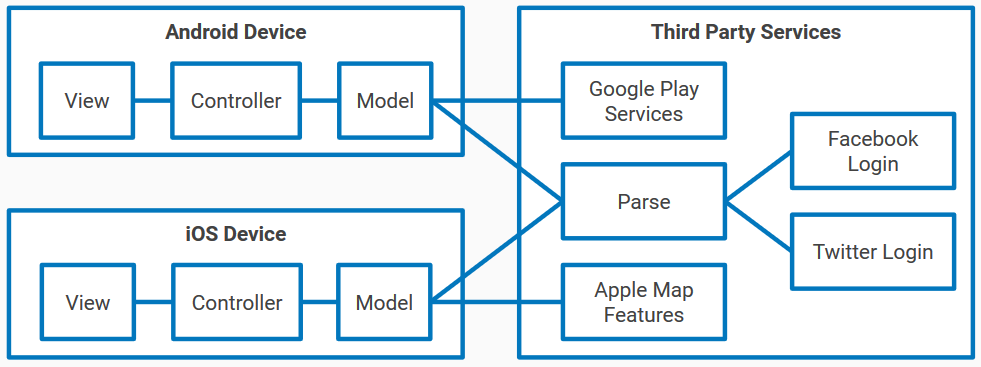
\includegraphics[width=0.75\textwidth]{designpictures/ModuleFlowDiagram.png}
\end{center}
\caption{Basic System Flow Diagram \label{ModuleFlowDiagram}}
\end{figure}

\section{Technologies Overview}
Some technologies used in the creation of Crowd Control are Google Play Services, Apple Map Features, and Parse.

\subsection{Google Play Services}
	\subsubsection{Description}
	Google Play Services contains the native android API for mapping features. With this it allows for commiuncation between a map and your gps location along with other mapping features.
\newline
REFERENCE LINK:  \url{https://developers.google.com/android/guides/setup}
	\subsubsection{Usage}
	Google Play Services will be used on the Android device as the default map. We chose to go with Google Play services to give android users a more native feel when it comes to using the maping features. This allows for a less intrusive feel when it comes to using Crowd Control. This will be used for displaying your location on a map, displaying other users in your group on a map, and displaying event suggestions on the map.

\subsection{Apple Map Features}
	\subsubsection{Description}
	Apple Map Features is the native iOS API for mapping features. With this it allows for comminucaton between a map and your gps location along with other mapping features.
\newline
REFERENCE LINK: \url{https://developer.apple.com/maps/}
	\subsubsection{Usage}
Apple Map Features will be used on the iOSdevice as the default map. We chose to go with Apple Map Features to give iOS users a more native feel when it comes to using the maping features. This allows for a less intrusive feel when it comes to using Crowd Control. This will be used for displaying your location on a map, displaying other users in your group on a map, and displaying event suggestions on the map

\subsection{Parse}
	\subsubsection{Description}
	Parse is our backend database. It allows us to save information that is needed along with giving us a way to connect to both facebook and twitter.
\newline
REFERENCE LINK: \url{http://parse.com/}
	\subsubsection{Usage}
	Parse will be used to save informtion, group information, and avertisement information. It will be the main comminucation between devices and past user information




